\part{Introduction}

\section{MMT170817 -- a historical event}
On August 17\sp{th} 2017, the first binary neutron star merger event was observed through gravitational waves and electromagnetic signals. These observations pertain to a new paradigm of astronomy, namely \it{multi-messenger astronomy}. Hence, we will refer to the collection of these observations as MMT170817, for \it{Multi-Messenger Transient 170817}.

MMT170817 is the outcome of an extraordinary instrumental effort provided by each of the fields of this multi-messenger astronomy. The detection of gravitational waves has ground-breakingly entered the astronomical landscape in September of 2015, as gravitational waves from all three phases (inspiral, merger, ring-down) of the coalescence of a binary black hole were detected in the \it{two} interferometers of the LIGO Scientific Collaboration. After a total of five such two-instrument detections, the gravitational interferometer network was augmented with the French-Italian Virgo instrument on August 1\sp{st} 2017.

On August 17\sp{th}, a gravitational wave detection by this \it{three}-instrument configuration occured. This signal is associated with the inspiral phase of the merger of a binary neutron star. This joint detection allowed for the first-in-history astronomically significant gravitational wave triangulation of the source in the sky. This triangulation is given in terms both of sky-projected position and distance, drawing a three dimensional error box in the Universe. A prompt but meticulous optical search for a new electromagnetic source in this error box led to the first ever direct observation of a kilonova --~neutron-rich matter ejected from the system and which is the site of explosive nucleosynthesis~--, and of a strongly atypically-behaved multi-wavelength afterglow, the observation of which carries on at the time of writing. The observations of these electromagnetic counterparts and the identification of NGC4993 as the host galaxy of the event were done by a hitherto unseen joint effort from the astronomical community as a whole, mobilizing an impressive amount of ground-based instrumental resources.

With a slight delay with respect to the gravitational wave determined time of merger, the Fermi Gamma-ray Space Telescope and the INTEGRAL space observatory detected a weak short gamma ray burst, itself triangulated to a sky-position consistent with that indicated by the gravitational waves and the other electromagnetic counterparts.

The gravitational, gamma ray and other counterparts of this event are unambiguously associated, and thus are the multi-messenger manifestation of the first binary neutron star merger witnessed directly.

\section{Description of the multi-messenger observations}

\subsection{GW170817: gravitational waves from the inspiral phase}

The inspiral phase gravitational waves (GW) were detected for the $\sim$~3000 last orbits of the binary\footnote{The information contained in this subsection was synthesized from the GW detection publication \cite{23}.}. This signal GW170817, reproduced Figure \ref{gw}, lasted $\sim$~100~s and ended at 12:41:04.4~UTC. It is the loudest gravitational wave signal detected yet, with a signal-to-noise ratio of 32.4. The GW signal infers masses in the ranges of 0.86~--~1.36 $\Ms$ and 1.36~--~2.26 $\Ms$ for the two initial components (at 2$\sigma$). Given the ranges of measured galactic black hole masses, which are substantially higher than these, and the measured masses of some galactic binary neutron stars, which are consistent with these, a binary neutron star is the most likely nature of the GW progenitor. This is further supported by the detection of electromagnietic counterparts to this GW signal, indicating the presence of matter in the circum-merger environment after the merger, and thus the unlikelyness of a black hole in the initial binary. Finally, the GW-inferred tidal deformability of the components of the binary are consistent with those derived from neutron star equations of state, and thus once again point to a binary neutron star for the progenitor of GW170817.

The Virgo detector did not measure a significant signal. This greatly constrained the localization of the source in the sky to a projected error box of 29~deg\sp{2}, and likely greatly decreased the duration of subsequent searches for electromagnetic counterparts.

The GW-inferred luminosity distance to the source is $40_{-14}^{+8}$~Mpc, making of the GW and short gamma ray burst the closest such events ever detected. This distance is further refined by combining GW data with EM observations of the host galaxy to $42.9\pm3.2$~Mpc. Similarly, the combination of the GW and EM data provides a viewing angle $\thetaobs$ (from our light-of-sight to the angular momentum of the binary) constrained to being less than 28~deg.

An essential feature of GW170817 is the non-detection of a postmerger ring-down signal, i.e. the gravitional radiation emitted by the remaining central compact object during its relaxation to its state of equilibrium. This non-detection signifies either that the corresponding radiation was not emitted, which would likely be the case if the remnant object is a neutron star, or that the signal was to weak to be picked up. Moreover, had the final object been a black hole, its ring-down signal would have peaked at frequencies well out of the detectors' sensitive bands, given the masses at hand. In any event, the nature of the final object is undetermined by the GW signal.

\fig{gw}{1.0}{Spectrogram of a combination of both LIGO interferometers' data from GW170817 (\cite{37}). Note the non-detection of a ring-down signal. The peak luminosity of the GW event is $\sim~9~\Ms c^2$/s (\cite{49}).}


\subsection{AT 2017gfo: the kilonova}
\label{kilonova}
The optical counterpart AT 2017gfo (IAU designation) was discovered $\sim$~11~h after the merger event\footnote{The information contained in this subsection was synthesized from the multi-messenger detection publication \cite{51}.}. It was located in the lenticular galaxy NGC4993 within the ESO~508 group of galaxies in Hydra. Upon discovery, the $r$ band magnitude was measured to $\sim$~17, equivalent to an absolute magnitude of --16.

In the following days, until dimming to non-detection limits of AT 2017gfo, spectra of the transient were measured. The time evolution of these spectra is illustrated Figure \ref{kn}. These are associated with thermal radiation of an optically thick mass of dynamical (or tidal) ejecta from the merger event. It is understood that the neutron-rich matter ejected by the merger event is the site of $r$-process nucleosynthesis, that is the synthesis of neutron-rich heavy nuclei by rapid neutron capture in a neutron-dense environment, and the subsequent decay of these nuclei to heavy elements such as the lanthanides and actinides. The decay of the nuclei are a heat source within the kilonova, and the extremely opaque medium composed of heavy nuclei insures its thermalization. What's more, the sudden decompression of this once-neutron-star material into the rarified external medium drives the rapid expansion of the ejecta.

This vision is further supported by the claim to the detection of atomic cesium and tellurium ($Z = 55$ and $52$) absorption lines in the transient's spectrum \cite{53}.

\begin{figure}
    \centering
    \begin{subfigure}
        \centering
        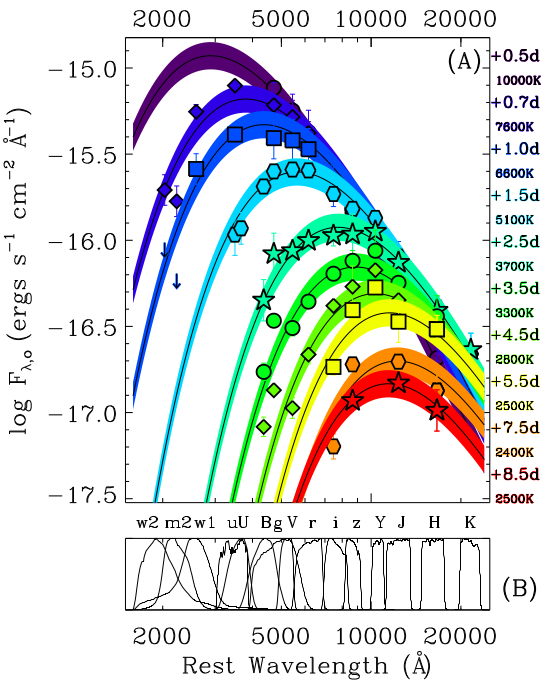
\includegraphics[width=0.48\linewidth]{kn}
    \end{subfigure}
    \begin{subfigure}
        \centering
        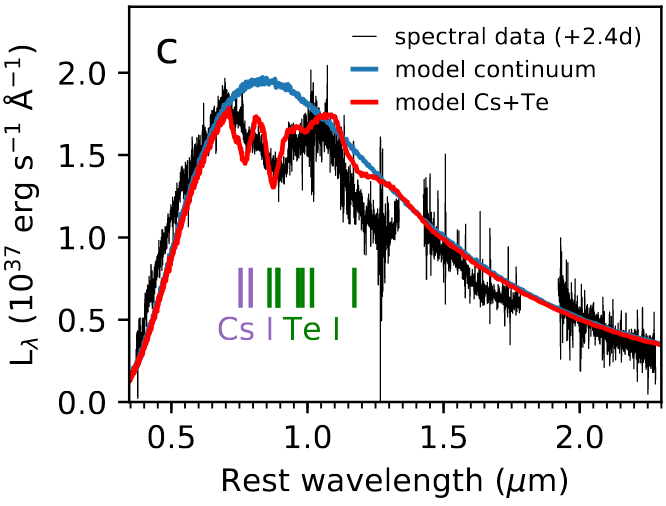
\includegraphics[width=0.48\linewidth]{cste}
    \end{subfigure}
    \caption{\it{Left:} Time evolution of the spectrum of AT 2017gfo (\cite{38}). \it{Right:} Visible and near-IR spectrum of the kilonova after 2.4 days, where Te and Cs absoption lines are clained to have been found (\cite{53}).}
    \label{kn}
\end{figure}

Some authors have argued in favor for two thermal components in the continuum spectrum of the kilonova \cite{57}. According to this vision, the redder component is more opaque due to the higher concentration of lanthanides ($Z = 57 \text{to} 71$) with respect to the bluer component. Also, the redder component would originate in the dynamical ejection of matter upon merger, whereas the blue component would occur within a neutrino-driven wind lifted above an accretion disk around the final central object.


\subsection{GRB170817A: the gamma-ray burst}
The gamma ray burst (GRB) event started 1.72~s after the GW data merger time\footnote{The information contained in this subsection and the next was synthesized from the GRB detection publication \cite{52}.}. Its duration was 2.0~s, placing it in the class of short GRBs\footnote{The distribution of GRBs according to their duration grossely seperates them in two classes: the \it{short} GRBs, with durations less than 2.0~s, and the \it{long} GRBs.} with a confidence level of $\sim$~72\%. GRB170817A's total isotropic-equivalent radiated energy was $\sim$~$10^{47}$~erg, around 4 orders of magnitude weaker that typical short gamma ray bursts, though photons with energies as high as 185~keV were emitted.

Moreover, it appears that the light curve of GRB170817A presents two successive components, one lasting 0.58~s, and a later second lasting 1.1~s. Spectrally, the first component resembles a typical non-thermal short GRB emission, and the second on the other hand is best fit by a thermal emission of temperature $\sim$~10\sp{7}~K (1 keV), though the significance of this spectral fit is debated and other spectral models are not excluded.

Furthermore, as illustrated in Figure \ref{yonetoku}, GRB170817A is an outlier of the $E_p$-$L_{\rm{iso}}$ relation, also know as the Yonetoku relation (\cite{35}). In this relation which is broadly respected by short GRBs, $E_p$ is the peak of the spectrum of the GRB emission at the moment of its peak --~also considered as the energy of the photons which carry the bulk of the energy of the GRB~--, and $L_{\rm{iso}}$ is the isotropic equivalent luminosity of the burst at this moment. According to the Yonetoku relation, they are positively correlated. Even when correcting for the possibly non-zero viewing angle, and placing the burst as seen closer to its axis, GRB170817A remains an outlier of the Yonetoku relation.

\fig{yonetoku}{0.7}{The Yonetoku relation for the Swift BAT 4 catalog bursts (black crosses, \cite{36}) and GRB170817A (red crosses, \cite{52}). The values of $E_p$ and $L_{\rm{iso}}$ that would have likely been measured for other viewing angles form a line in this diagram, and indicate that GRB170817A is an atypical event.}

These remarks indicate the \it{atypical} character of GRB170817A. More precisely, these remarks lead to interrogations on the emission processes responsible for GRB170817A. Standard understandings of GRBs imply relativistic jets and energy dissipation into gamma radiation therein. Are GRBs from neutron star mergers comprehensible in such standard models? Are they a particular case of these models? Or do they require a specific modelling? As GRBs arise from relativistic jets, they are observed as weaker if seen off-axis. Can GRB170817A's weakness be explained by this effect? In our work, we will not be concerned with these questions, as we will study the afterglow of MMT170817. Nonetheless, these are central questions for the future study of neutron star mergers and their link to the population of GRBs.

A few other weak GRBs have been observed in the past. An example is GRB980425 which stood out as an atypical event among long GRBs for its low luminosity. It was then found (\cite{50}) that the internal shock model allowed such events, provided the outflow be slower and less energetic.


\subsection{The afterglow signal}
\label{ags}
Counterparts in the X-ray and radio bands were detected to significant levels 9 days and 15 days post-merger. When the kilonova signal had sufficiently decayed at 150 days post-merger, an optical band afterglow was detected as emerging from the dimming kilonova signal.

The afterglow photometry points in these bands until $\sim$~250~d post-merger are reported Figure \ref{ag}. Among these photometry points, the latest ones --~and in particular those of the peak of the flux~-- were measured in the course of the work presented in this document. An essential feature of these afterglow light curves are their homothetic structure, i.e. their seems to exist a time-independent index $k$ such that for two frequencies $\nu$ and $\nu\p$, we have $F_\nu = \left( \frac{\nu}{\nu\p} \right)^k F_{\nu\p}$. From these light curves, we can already infer $k \sim -0.5$.

\fig{ag}{0.5}{Afterglow photometry points in various bands (\cite{29}). Notice the homothetical structure of the flux from band to band. In the optical band, the afterglow signal only appears after the dimming of the kilonova, and approximately coincides with the beginning of this work.}

As we will shortly see, this structure is a first indication of which radiation process is at play in the afterglow --~synchrotron radiation~--, and allows us to consider for our study the light curve of only one band.


Another important feature of this afterglow emission is that it is long-lived. Indeed, the radio flux increased steadily until $\sim$~160~d post-merger, then commenced a steady decrease and it still observed at the time of writing. A comparison of the afterglow of MMT170817 with some short GRB afterglows from the total Swift catalog can be done using in Figure \ref{remnants}. It is evident that MMT170817 is pecliar with respect of all of these.

\fig{remnants}{0.7}{Some afterglows from the Swift catalog (blue lines, X-ray data, \cite{61}). A quick comparison with the afterglow of MMT170817 on Figure \ref{ag} shows that this afterglow is like none other.}

\section{Goal of this work: an insight on the geometry and dynamical structure of the remnant of MMT170817 through its afterglow}

The merger of a binary neutron star is a complex phenomenon. It implies various physical components (compact objects, jets, ejectas, winds) which are subject to many dynamical and radiative processes (shock formation, nuclear processes, synchrotron emission, etc.). A coherent description of the binary neutron star merger phenomenon, from the inspiral phase to the electromagnetic afterglow, is still to be found. Most likely, the combination of all the multi-messenger observations from a large number of events will be necessary to obtain this accurate description, as each signal bares the signature of the state of the phenomenon at different times.

During the merger event, matter is ejected from the system. It can be ejected by the collision of the neutron stars, by tidal forces before the merger, by the relaxation activity of the remaining central objet after the merger, etc. This matter may assume various geometries --~spherical, jet-like~--, and be ejected with different dynamical structures --~all at once with a single velocity, with a distribution of velocities, in many ejection phases, etc. This matter, if ejected with speeds larger than that of sound, will form a shock in the circum-merger medium, producing an afterglow emission to the merger event, driven by an energized population of electrons at the shock front.

Thus, the afterglow emission holds information on the state of the system at late times, and is a first step one may take to approach the event in its entirety. This work is a spark for the study of the merger of binary neutron stars. Focusing on the afterglow, we will through modelization attempt to a first understanding of this event. In particular, we will search a coherent description of the outflow of matter responsible for the afterglow --~its geometry and dynamical structure~-- and give some first answers to the question of whether a relativistic jet was produced during the event.

The questions this work adresses are thus the following:

\begin{enumerate}
	\item What is the geometry and the structure of the outflow of matter responsible for the afterglow?
	\item What are the characteristics of the circum-merger medium which this outflow penetrates?
	\item By which means is the kinetic energy dissipated into the afterglow radiation?
	\item Was a relativistic jet produced in the merger event? This is a fundamental question the answer to which is a first step in linking the population of short GRBs with the phenomenon of binary neutron star mergers.
	\item Which afterglow signals would we have seen, had we seen the event from a different viewing angle?
\end{enumerate}
